%!TEX root = ../template.tex
%%%%%%%%%%%%%%%%%%%%%%%%%%%%%%%%%%%%%%%%%%%%%%%%%%%%%%%%%%%%%%%%%%%%
%% chapter3.tex
%% NOVA thesis document file
%%
%% Chapter with a short laext tutorial and examples
%%%%%%%%%%%%%%%%%%%%%%%%%%%%%%%%%%%%%%%%%%%%%%%%%%%%%%%%%%%%%%%%%%%%
\chapter{System model and design options}
\label{cha:systemModel_and_designOptions}

In this chapter we present the architecture overview of the system model for our solution. We introduce an architecture model that is able to assure confidentiallity and integrity, according to our adversary model, to the execution of unmodified applications that run sensitive data on cloud computing servers, by leveraging trusted computing tecniques provided by both software and hardware, inside \gls{tee}s. All this without crippling too much the performance levels of the overall system.

The system model defined in the next chapter is later described in the thesis with greater detail, as an implementation prototype capable of applying this theoretical concepts described before.

In Section \cite{sec:systemModel_overview} we describe a general overview of the system as a whole, 

TODO


-----
In Section
4.1 and Section 4.2 we describe the bigger picture and what are the assumptions that
we based ourselves on the creation the system. After, we will look into more detail on
the components and operations that our system works with in Sections 4.3, 4.4 and 4.5.
We will also look onto the Protocols and Processes necessary to start and maintain our
solution in Sections 4.6 and 4.7. At last, we finish with a Summary in Section 4.8.



\section{System model overview} % (fold)
\label{sec:systemModel_overview}

Our solution can be seen in figure \cite{fig:systemModel}, which is a macro overview of the system. As we can see in the figure, the solution we focused on implementing can be divided in two sides, client side and server side, where clients interact with the system, where an in-memory \gls{kvs} is running inside a cloud provider, protected inside a \gls{tee}. 

To make that interaction, a client first interacts with a proxy that works as an intermediator, which is also running on top of trusted hardware. It acts as a single point of access and is responsible of authenticating everyone that wants to interact with the system. It is also in charge of the attestation process of the instances running inside the server, to check if they are trustable and going to execute as they are expected to. 


\begin{figure}[htbp]
	\centering
	{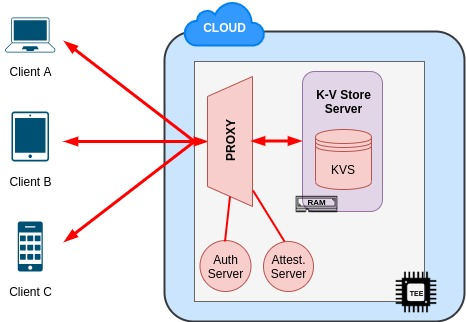
\includegraphics[width=0.7\linewidth]{systemModel}}
	\caption{Overview of the System Model}
	\label{fig:systemModel}
\end{figure}

TODO - 

1)talk more about attestation



\section{Threat model and security properties} % (fold)
\label{sec:threatModel_and_securityProperties}

Our solution is designed to offer privacy-enhanced guarantees in protecting data confidentiality, while also ensuring integrity and completeness of results returned to the clients, and we do it by ensuring that the sensitive data never runs in plaintext. By doing so, our system model protects from attackers with intentions of accessing sensitive data and taking advantage and value from it, regardless if the attack is coming from the inside or the outside the cloud system.


\subsection{Adversarial model definition}

We focused on two types of malefic users: 1- Users that attack the system and find a way of getting access to high privileges, such as capacity to manipulate the host \gls{os} and other low level components, through which he can get access to data running, and 2-  Honest-but-curious users, which already have higher privileges and can snoop on private data so they can learn and take advantage of it.

TODO - what is out of scope
1- client
2- proxy
3- storage
write something like: it is important to refer that with this prototype we dont offer storage confidentiality, because we only considered in-memory \gls{kvs}s, although this is easily added to the system because redis can be configurated to work with persistent memory bla bla bla

\subsection{Countermeasures for privacy-preservation}

Since our objectives are pointed towards an isolated system capable of offering security
and privacy properties, we depend a lot on isolation techniques to make this possible,
provided by both hardware and software (containers).

As for hardware isolation, we looked at \gls{tee} technologies capable of assuring computation and storage security to our system's data during runtime.

Also, to grant an extra layer of isolation and to ensure privacy to the data in each element of our model we opted to use containerization, as a way to keep them independent and the system modular and scalable, enabling ease in the deployment of software running inside the containers, whether it is an \gls{os}, a library
\gls{os} or even entire applications. Running our system inside containers allows it to be deployed, in a very similar way, whether running locally or in the cloud, which came to be very handy in the implementation process. 

We didn't recurr to persisting data in storage to relieve some of the complexity that can arise due to the use of containers.





\section{SGX Enabled REDIS solution} % (fold)
\label{sec:sgx_redis_solution}

Our solution, which is based on the system model introduced in Section \cite{sec:systemModel_overview}, can be divided in two pieces. One being the Client-side, responsable for making requests to the system, and other being the system itself, or the server. 

The system, which we run in a Cloud server, can be composed in two subdivisions: a Proxy server, and a \gls{kvs} server, all running inside containers on top of a \gls{tee}. 

As for the Client-side, we only considered them to be benchmark applications, and not entire web applications, with only the intent to evaluate the system for our experimental analysis shown later on this dissertation.

TODO - say if the client are considered trusted or not


\subsection{System Architecture and Components}

The system itself runs on top of a \gls{tee}, that being Intel-\gls{sgx}. As we studied, applications can't simply be placed on top of a \gls{tee}, in this case \gls{sgx}, and expect them to perform the same way as they do without this extra layer of security. 
Hence, we opted to use SCONE \cite{ssec:scone} as a way to run our system. It allowed us to run the server components on containers capable of running with effectiveness on top of \gls{sgx}, with properties that ease the downsides of \gls{tee}s. 

For the KVS server, we used the Redis \gls{kvs} that can be used with different configurations, offering multiple strenghts to the execution and storage of data, especially if run in Cluster mode, offering scalability, fault-tolerance and even increase of performance if each replica of the cluster is set in independent machines.
 
In our solution we deployed Redis instances configurated in Standalone mode, Master-Slave mode and Cluster mode, as a way to test the behavior of the system. It's also important to note that each Redis replica had their own container, regardless which configuration it was set to execute. 

The Standalone version of Redis is the simplest configuration that a Redis instance can run. It offers the properties of a single Redis database. It is very simple, very stable and easy to maintain, and it serves as the reference point of the evaluation of the system.

The Master-Slave configuration offers replication and eventual consistency of data, with writes only possible in the Master node, and read-only Slave nodes.

As for the Cluster, although it is the most complex configuration, beyond replication and consistency, it also adds huge scalability possibilities to the system.


As for the proxy, although it is an extra layer of overhead, we thought it is worth the "investiment" for the fact that it can serve multiple purposes. 
First of all, it is used as a gateway for the system to communicate with the outside components.  It acts as a single point of access, enabling the rest of the system to scale, adding no extra complexity to the client-side. Thus, all the client has to do is reach the proxy endpoint, while the redirection logic to the server instance that will manage the request will be done by the proxy itself. Adding to that, it allows the system to only have a single firewall, instead of configuring one for each KVS instance.

The proxy is also the responsible of authenticating anyone from outside that wants to interact with the system. Redis itself also has the possibility to configure authentication for each replica, but that option would add an extreme layer of complexity that we do not want, due to the fact each replica needs to be configured individually. Therefore, if we start to scale the number of Redis instances, the complexity of that task everytime a new user is being granted permission to access the system will be extreme. Thus, this problem is solved by having an authentication server that communicates with the proxy, since the configuration only needs to happen once for the proxy to know which users are allowed to access the system.

Finally, we implemented the proxy to be in charge of attestating the components running in the rest of the server. 

All the communications between the components that compose the server-side are secured by TLS over HTTP, as a way to keep confidentiality of the data during communications all over the system.

\begin{figure}[htbp]
	\centering
	{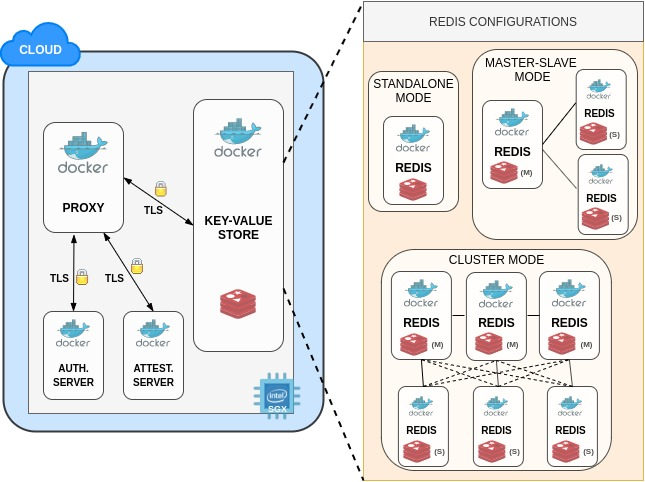
\includegraphics[width=0.7\linewidth]{systemWithMoreContext}}
	\caption{Overviewing the server-side of the solution}
	\label{fig:serverside_systemModel}
\end{figure}

  
\subsection{Client-Side Operations}

For the client-side, as mentioned in the beginning of this section, we only considered benchmarks. We use these benchmark clients with the single purpose of evaluating the system by making simple requests to the API (the Proxy), while calculating metrics that we found essential to use in our pratical evaluation of the solution. 

The communication process with the Server-side of the solution is also made through TLS over HTTP.

\begin{figure}[htbp]
	\centering
	{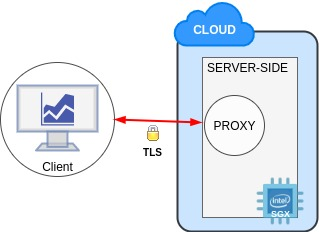
\includegraphics[width=0.4\linewidth]{client_serverside}}
	\caption{Communication between client and server}
	\label{fig:client_serverModel}
\end{figure}

% section importing_images (end)
\section{Open Design Issues} % (fold)

Looking back at our model, we can think that the whole availability of the system depends highly on the single proxy instance working as entry-point for the whole system, and so all can be compromised if it fails to work, or just stops working for some reason. And this assumption is true. 
Replication of the proxy instance can be seen as a measure to mitigate this problem, and although this is doable, we considered it to be out of scope for what we choose to evaluate in this thesis. 



\section{Summary} % (fold)



\section{Implementation Guidelines} % (fold)

For the development phase of this dissertation, and as we mentioned before in \ref{sec:objectiveAndContibutions}, we considered the following guidelines:

\textbf{Key-Value Store}: we opted for REDIS (v5.0.7) due to being the most popular \gls{kvs} at the moment, as we can see in \cite{rankingKVStores}. Adding this to the fact that it fits our system needs, we thought that an exhaustive study over this technology running in a dependable system would be an interesting contribution.

\textbf{Trusted Execution Environment}: as mentioned before, we choose to go with Intel-\gls{sgx} (\ref{ssec:intelsgx}), since it offers the possibility to isolate code inside multiple enclaves while executing on commodity hardware. Thus, we can run each node of our \gls{kvs} cluster inside of an individual enclave, assuring confidentiality and privacy of the data during runtime.

\textbf{OS library}: to run unmodified applications on top of Intel-\gls{sgx}, we picked Graphene-SGX (\ref{ssec:grapheneSGX}) as it was proven to be able to keep decent levels of performance in a system.

\textbf{Containerized OS Virtualization}: we choose Graphene-SGX Secure Container (GSC) \cite{gsc} due to being an open-source container system where an application can be protected by Intel-\gls{sgx} while running inside a Docker \cite{docker} container. We thought it to be a good way of adding an extra layer of isolation to the execution of each \gls{kvs} instance, while still running with the benefits of Graphene-SGX and Intel-\gls{sgx}.

\textbf{Cloud Infrastructure}: OVH \cite{ovhCloud} was the cloud provider chosen, mainly due to the fact that it supports \gls{sgx} in its dedicated servers.

\textbf{Operating System}: as for the \gls{os}, we are going to work with Ubuntu Linux, with the support of Linux-SGX \cite{linuxSGXwebsite} to run it on top of Intel-SGX technology. The use of Intel-SGX SDK \cite{linuxSgxSDK} for Linux makes it possible for us to manipulate the enclaves. Finally, we will use Linux SGX Driver \cite{linuxSGXDrivers}, which will manage the drivers of Linux-SGX already mentioned.

As for other technologies, the system will be written in Java. 
The client layer will consist of a benchmark application provided by both REDIS Benchmark and Yahoo! Cloud Serving Benchmark (YCSB) \cite{ycsb}. 
Jedis (REDIS java client) \cite{jedis} will also be used in the processing layer, as the client to our \gls{kvs} instances, along with Lettuce \cite{lettuce} for thread-safe operations when working with a \gls{kvs} cluster.


\section{Validation and Experimental Analysis} % (fold)
\label{sec:floats_figures_and_captions}

To validate and evaluate our solution, we created a set of tests for each metric we choose to evaluate. The analysis will be done between two scenarios, one being a regular, already existing, version of REDIS \gls{kvs}, while the other being a version of our TREDIS solution.

For this purpose we will be comparing the following metrics:

\begin{itemize}
	\item \textbf{Attestation latency:} time of the attestation between the client and REDIS;
	\item \textbf{Performance:} throughput and latency over the REDIS \gls{kvs};
	\item \textbf{Scalability:} scalability conditions under different client-workloads;
	\item \textbf{Resource allocation:} use of resources during runtime, including memory, CPU usage, I/O and energy.
\end{itemize}

In order to evaluate these metrics, we will analyze scenarios where:

\textbf{1)} the size of the datasets used in the benchmark tools scale up (e.g: 1,000 entries and 100,000 entries);

\textbf{2)} the typology of operations made over the \gls{kvs} varies: ratio of read/write operations (e.g: 20R/80W, 50R/50W, 80R/20W).


For the TREDIS solution running in an OVH cloud, our experimental evaluation will be conducted in development and deployment nodes with the following aspect:

\textbf{Processor:} Intel 2x Xeon Silver 4214 - 24 c / 48 t - 2.2 GHz / 3.2 GHz

\textbf{Memory:} 192 GB

\textbf{Storage:} NVMe, SATA disponível

\textbf{Public Network:} more than 1Gb/s

\textbf{Private Network:} more than 2Gb/s

\textbf{OS:} CentOS 7.4.1708 64 bits or Ubuntu 18.4 LTS Server 64 bits



% \subsection{Inserting Figures Wrapped with text} % (fold)
% \label{ssec:inserting_images_wrapped_with_text}
% 
% You should only use this feature is \emph{really} necessary. This means, you have a very small image, that will look lonely just with text above and below.
% 
% In this case, you must use the \verb!wrapfiure! package.  To use \verb!wrapfig!, you must first add this to the preamble:
% 
% \begin{wrapfigure}{l}{2.5cm}
%   \centering
%     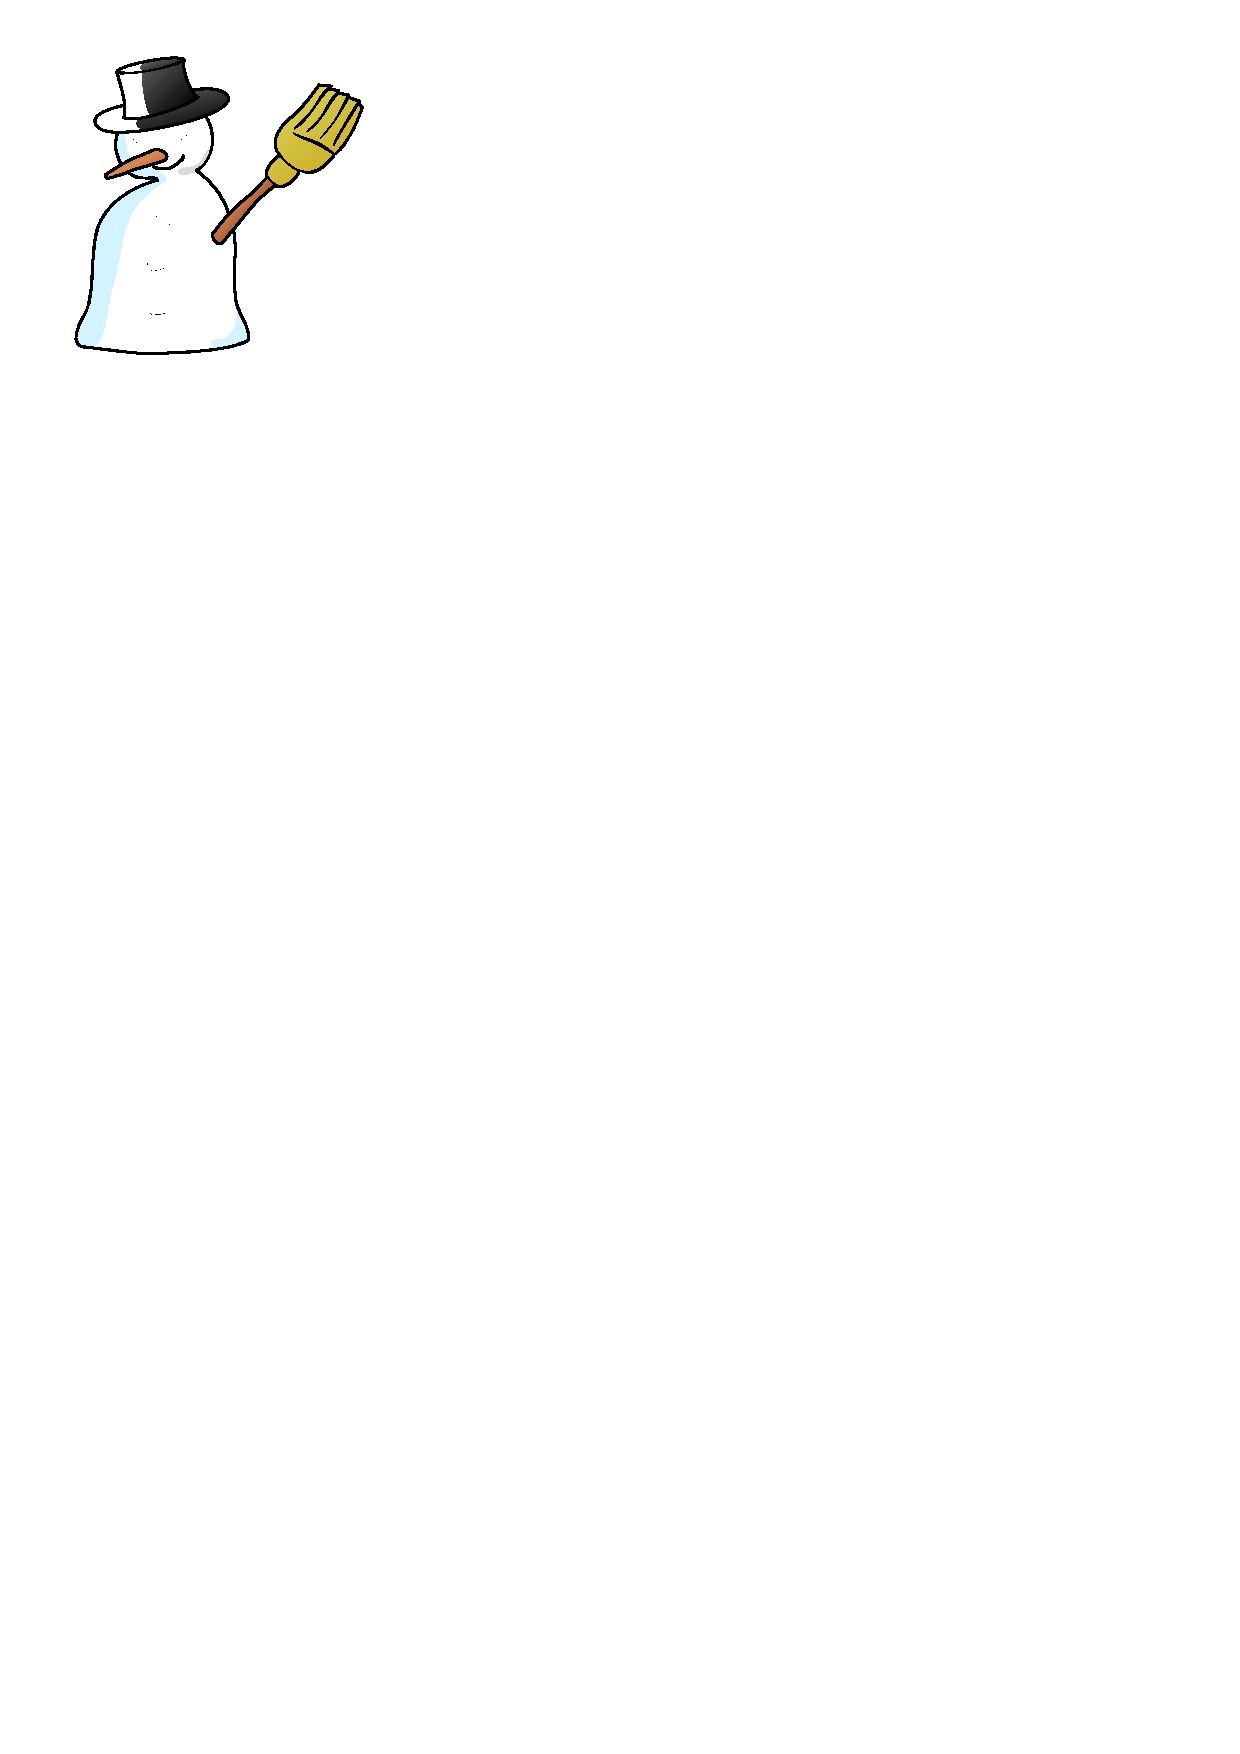
\includegraphics[width=2cm]{snowman-vectorial}
%   \caption{A snow-man}
% \end{wrapfigure}	
% 
% \noindent\verb!\usepackage{wrapfig}!\\
% This then gives you access to:\\
% \verb!\begin{wrapfigure}[lineheight]{alignment}{width}!\\
% Alignment can normally be either ``l'' for left, or ``r'' for right. Lowercase ``l'' or ``r'' forces the figure to start precisely where specified (and may cause it to run over page breaks), while capital ``L'' or ``R'' allows the figure to float. If you defined your document as twosided, the alignment can also be ``i'' for inside or ``o'' for outside, as well as ``I'' or ``O''. The width is obviously the width of the figure. The example above was introduced with:
% \lstset{language=TeX, morekeywords={\begin,\includegraphics,\caption}, caption=Wrapfig Example, label=lst:latex_example}
% \begin{lstlisting}
% 	\begin{wrapfigure}{l}{2.5cm}
% 	  \centering
% 	    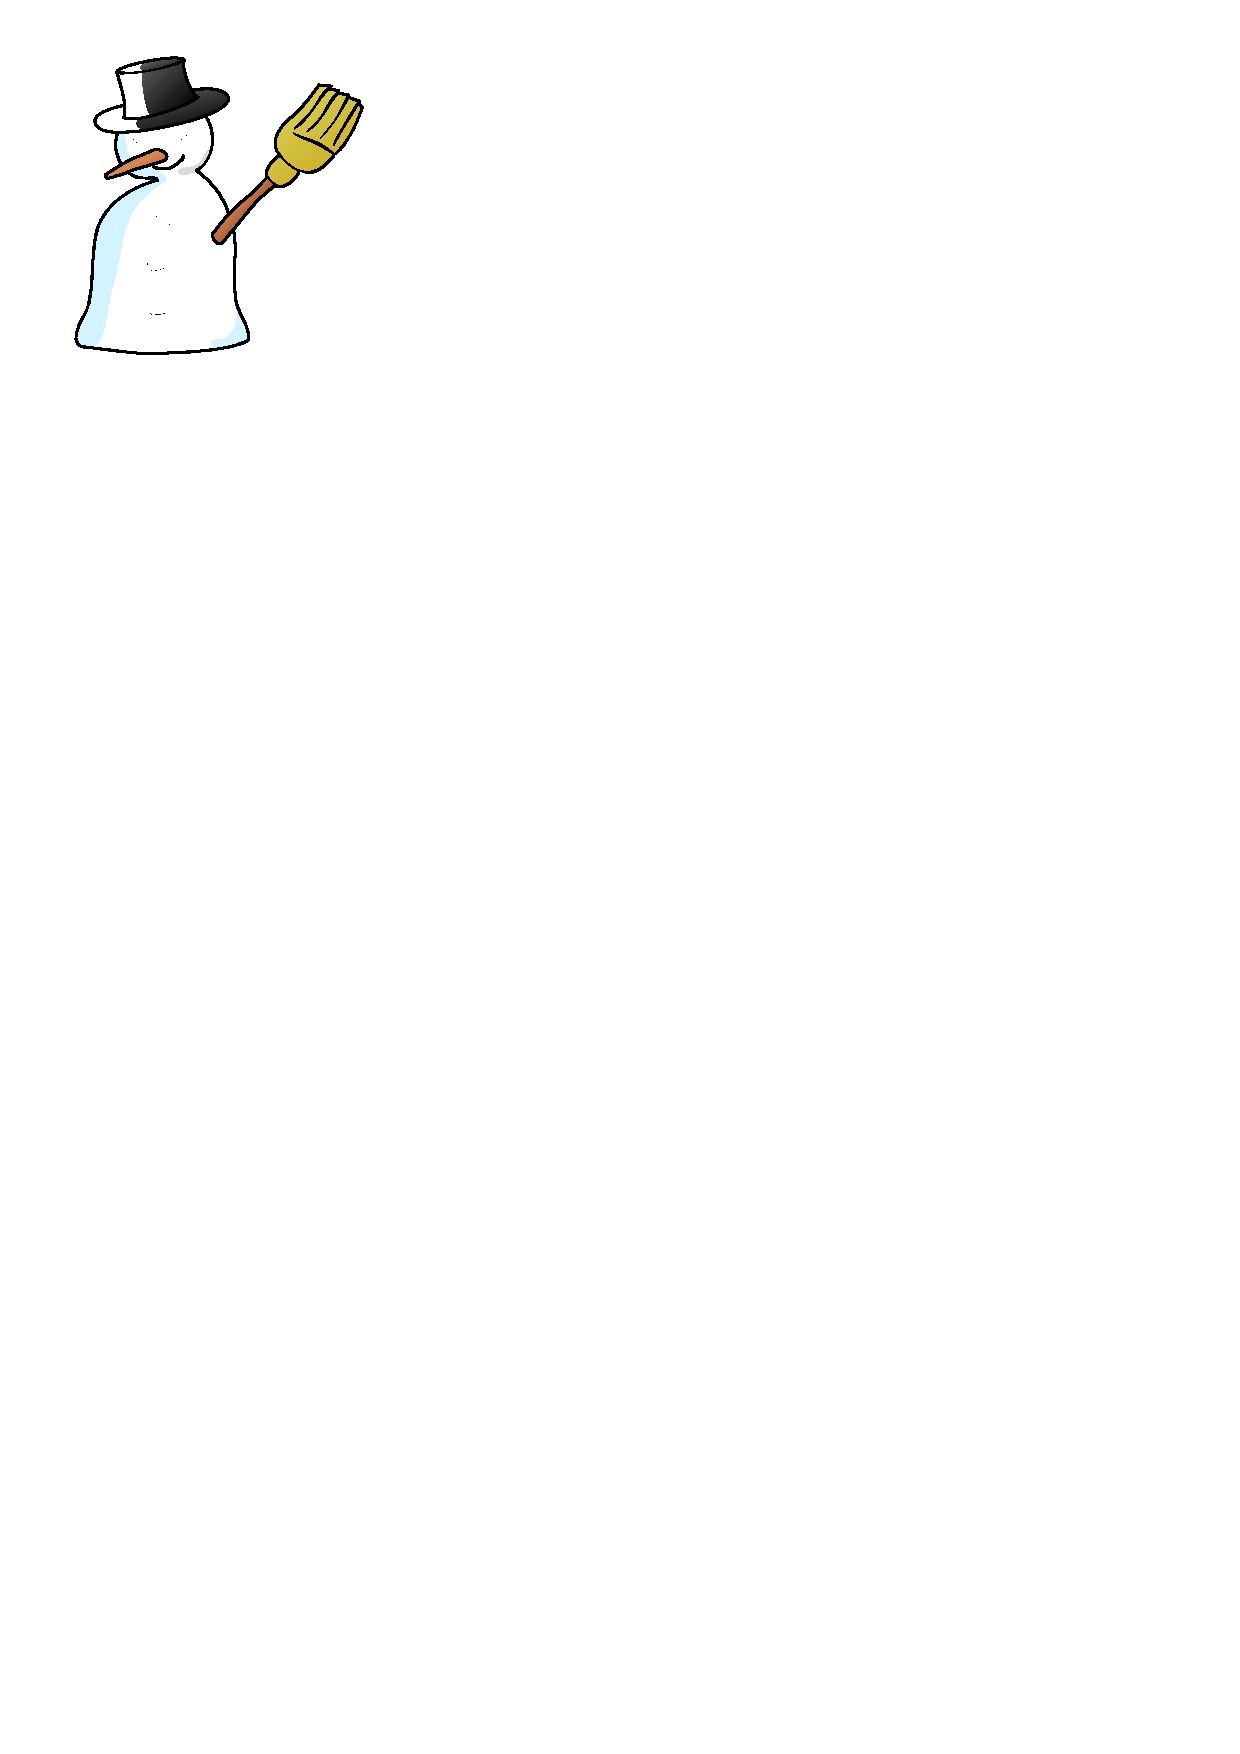
\includegraphics[width=2cm]{snowman-vectorial}
% 	  \caption{A snow-man}
% 	\end{wrapfigure}	
% \end{lstlisting}

% subsection inserting_images_wrapped_with_text (end)

% section floats_figures_and_captions (end)

